\setcounter{figure}{0}
\setcounter{table}{0}
\setcounter{lstlisting}{0}

\chapter{Introducing OpenGL}
\label{opengl}
\minitoc

\textit{OpenGL} is designed as a software interface to the graphics 
hardware on your computer. It defines a platform-independent API;
the API is then implemented in software and/or hardware for 
various machine architectures. The advantage is that OpenGL 
programs are easily portable to a variety of computers.
\\
OpenGL provides basic commands to support rendering. 
In particular, it doesn't provide functionality to support
windows or user interaction (like keyboard presses or mouse 
actions); these features are provided by a separate library called
\textit{GLUT} (the OpenGL Utility Toolkit). GLUT also provides some 
higher-level features, such as more complex geometrical objects.
\\
OpenGL is a state machine, which means that you specify various 
states or modes which remain in effect until changed.
Each command that is executed is carried out within the current 
state. States include things like the current window (where
drawing will appear), colour, viewing and projection matrices, 
drawing modes, positions and characteristics of lights,
materials, and features. These elements will not be introduced 
throughout this document, as they are already explained in
various tutorials \cite{opengl:brieftutorial} o manual books 
\cite{opengl:redbook}.
\\
Nevertheless, it is important to keep the idea of a 
`state machine' in mind as you work with OpenGL in order to 
understand the effects of a given command. The current state 
is not reset when a function starts or ends; the current state
is in effect until something changes it, regardless of where 
in the program the next thing is. 
\\
In the following, we are going to analyse some peculiar 
aspects of OpenGL. Anyway, this chapter is not intended 
to be an exhaustive guide to OpenGL programming 
- like \cite{opengl:distilled} and \cite{opengl:redbook} - but,
instead, as a collection of short how-to regarding the 
aspects of OpenGL which we have dealt with the most 
during our work. 

\clearpage
\section{Some notes on OpenGL}
\label{opengl:opengl_notes}

One of the design target of OpenGL was to made its API portable 
among multiple architectures. In order to do so, OpenGL 
designers decided not to make use of polymorphism and inheritance 
when they had to provide multiple versions of the same command 
taking different parameters. They used, instead, the following scheme:

\begin{verbatim}
    glCommandName{NTd}()
\end{verbatim}

that is, every OpenGL function is preceded by \texttt{gl} and can be 
followed by

\begin{itemize}
  \item \texttt{N} \\
    the number of parameters the function takes
  \item \texttt{T} \\
    the parameters type
  \item \texttt{d} \\
    if present, it states that the function takes pointers as arguments
\end{itemize}

For example, the \texttt{glVertex} can be invoked as:

\begin{itemize}
\item \texttt{glVertex2i(1, 3)}
\item \texttt{glVertex2f(1.0, 3.5)}
\end{itemize}

As you might have observed from the simple example above,
OpenGL commands use the prefix `gl' and initial capital letters
for each word making up the command name (`glClearColor()', for
example). Similarly, OpenGL defined constants begin with `GL\_', use all
capital letters, and use underscores to separate words (for example,
'GL\_COLOR\_BUFFER\_BIT').
\\
You might also have noticed some seemingly extraneous letters appended to
some command names (for example, the `3f' in `glColor3f()' and `glVertex3f()').

\subsection{The Depth Buffer}
\label{opengl:opengl_note:depth_buffer}

When drawing up a scene with OpenGL, the order in which polygons are drawn
greatly affects the blended result, especially when it comes to 3D.
\\
The depth buffer keeps track of the distance between the viewpoint and 
the portion of the object occupying a given pixel in a window on the 
screen; when another candidate colour arrives for that pixel, it's drawn 
only if its object is closer to the viewpoint, in which case its depth
value is stored in the depth buffer. With this method, obscured (or hidden)
portions of surfaces aren't drawn and, therefore, aren't used for
blending.
\\
In order to enable the use of the depth buffer, the 
\texttt{glutInitDisplayMode()} can be used, passing the 
GLUT\_DEPTH macro as an argument.

\subsection{OpenGL viewing model}
\label{opengl:opengl_note:viewing_model}

OpenGL not only provides function to specify models for 
three-dimensional objects but also allows to specify the 
position for each of the models we want to display in a 
scene and also the point from which to view the scene.
\begin{figure}[!h]
  \begin{center}
    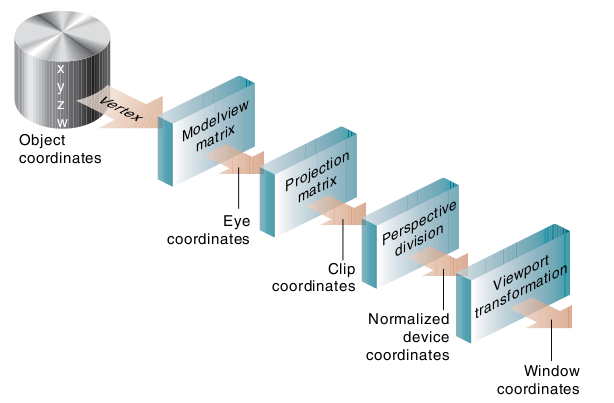
\includegraphics[width=300pt]{img/openGLpipe.png}
    \caption{The OpenGL pipeline}
    \label{fig:openglpipe}
  \end{center}
\end{figure}
\\
The transformation process used to produce a scene for viewing 
is analogous to taking a photograph with a camera (in fact, it 
is often addressed as \textit{the camera analogy} 
\cite{opengl:cameraanalogy}) 
and consists of four steps, known as
\textit{the OpenGL pipeline} (see figure \ref{fig:openglpipe}).
\\
At the beginning of the pipeline, we have the \textit{raw} 
coordinates of the models we want to put on the scene. Such 
coordinates are then multiplied by the a 4x4 \textbf{modelview} 
matrix, that is, a matrix that stores both \textit{model} and 
\textit{viewing} transformations and which elements have been set 
accordingly to \textit{actually} where to place items in the scene.
\\
The second step involves the \textbf{projection} matrix, 
which is applied to the incoming object coordinates to define a 
viewing volume. Of course, objects outside this volume are clipped 
so that they are not drawn in the final scene. 
\\
In the last two steps of the pipe, incoming coordinates are transformed 
into actual two-dimensional window coordinates and other stuff, such as 
the light intensity for each pixel, are calculated according to depth.

\subsection{Matrix transformations}
\label{opengl:opengl_note:matrix_transfor}

To edit the \textbf{modelview} and \textbf{projection} matrices, OpenGL 
provides quite a lot of functions: some of them are 
\textit{general purpose}, that is, they can be used to edit both of them, 
others are specifically intended to edit either the modelview or the 
projection matrix.
\\
The most used \textit{general purpose} functions are 

\begin{itemize}
\item \texttt{glMatrixMode(GLenum mode)} \\
  \textit{mode} specifies which matrix is the \textit{current}
  matrix, that is, the matrix that is to be edited by following
  functions
  
\item \texttt{glLoadIdentity()} \\
  sets the \textit{current} matrix to be 4x4 identity matrix
\end{itemize}

For what concerns editing the \textbf{modelview} matrix, OpenGL 
provides a set of functions that allows the specifying of the 
transformations one would like to apply without manually 
editing the modelview matrix. The most used are 

\begin{itemize}
\item \texttt{glTranslate(TYPE x, TYPE y, TYPE z)}\\
  Multiplies the current matrix by a matrix that moves 
  (translates) an object by the given x-, y-, and z-values 
  (or moves the local coordinate system by the same amounts)

\item \texttt{glRotate(TYPE angle, TYPE x, TYPE y, TYPE z)} \\
  Multiplies the current matrix by a matrix that rotates an 
  object (or the   local coordinate system) in a counterclockwise 
  direction about the ray from the origin through the point 
  (x, y, z). The angle parameter specifies the angle of rotation in degrees.
\end{itemize}

Two examples are shown in figures \ref{fig:gltranslate}, \ref{fig:glrotate}:
the first one shows the effects of invoking \texttt{glTranslatef(0.0, 0.0, -5.0)} 
on the view, while the second one shows how to rotate a model of 45 degrees 
invoking \texttt{glRotatef(45.0, 0.0, 0.0, 1.0)}.

\begin{figure}[!h]
  \begin{center}
    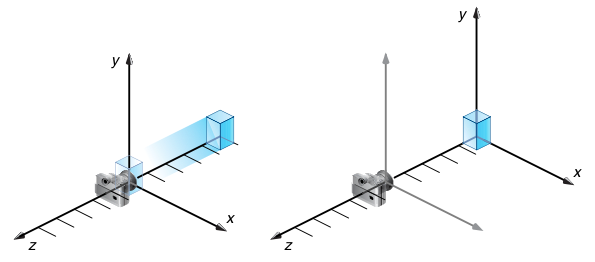
\includegraphics[width=300pt]{img/gltranslate.png}
    \caption{A view transformations by means of a glTranslate invocation}
    \label{fig:gltranslate}
  \end{center}
\end{figure}

\begin{figure}[!h]
  \begin{center}
    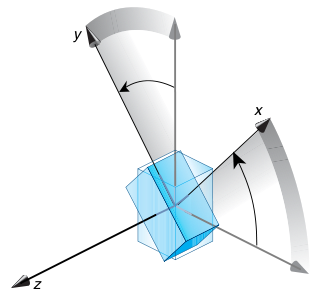
\includegraphics[width=150pt]{img/glrotate.png}
    \caption{A model transformation by means of a glRotate invocation}
    \label{fig:glrotate}
  \end{center}
\end{figure}

\clearpage
\section{Setting up a texture}
\label{opengl:setting_texture}
\lstset{language=C++}

According to \cite{opengl:distilled} \textit{texture mapping 
is a concept that takes a moment to grasp but a lifetime 
to master.}
\\
As for our work, we were simply interested in drawing an 
image as the background of a window. It is not a complex 
task but, it could be very tricky, especially when one 
does not have a deep understanding of what is happening 
\textit{under the hood}.
\\
OpenGL provides 1D, 2D and 3D textures. A 2D texture is enough for our
purposes.
\\
There exists a well-defined sequence of actions to draw a texture 
into an OpenGL application. Such a sequence made of the following steps:

\begin{enumerate}
\item obtain an unused texture object identifier with \texttt{glGenTextures()}, 
  and create a texture object using \texttt{glBindTexture()}
\item set texture-object state parameters
\item specify the texture image using \texttt{glTexImage2D()} 
  or \texttt{gluBuild2DMipmaps()}
\item before rendering geometry that uses the texture object, 
  bind the texture object with glBindTexture()
\item before rendering geometry, enable texture mapping
\item send geometry to OpenGL with appropriate texture 
  coordinates
\end{enumerate}

Let us show an example of how to take a preloaded image, binding it 
to a texture and draw it as the background of a window. First of all, 
we would like to define a helper structure which we will call \texttt{Image}
to store the actual image and its size.

\begin{lstlisting}[caption={The Image structure}, label={code:image}, frame=trBL]
struct Image {
  unsigned long sizeX;
  unsigned long sizeY;
  char * data;
};

typedef struct Image Image;
\end{lstlisting}

Now, let us suppose to have defined a \texttt{ImageLoad()} function 
that loads an image from disk and returns an object of class \texttt{Image}. 
Let us see how to put in code the procedure described above:

\begin{lstlisting}[caption={Texture example}, label={code:texturemapping}, frame=trBL]
  Gluint * texture;
  Image * image;
    
  // allocate space for the image
  image = (Image *) malloc(sizeof(Image));

  if (image == NULL) {
    // ERROR!
    exit(0);
  }

  // load image from disk
  if (!ImageLoad("image.bmp", image)) {
    exit(1);
  }        

  // obtain an unused texture object
  glGenTextures(1, texture);

  // Bind 2d texture (x and y size)
  glBindTexture(GL_TEXTURE_2D, * texture);   

  // now let us set up some state parameters:
  // scale linearly when image bigger than texture
  glTexParameteri(GL_TEXTURE_2D, GL_TEXTURE_MAG_FILTER,
                                 GL_LINEAR);
 
  // scale linearly when image smaller than texture
  glTexParameteri(GL_TEXTURE_2D, GL_TEXTURE_MIN_FILTER,
                                 GL_LINEAR); 

  gluBuild2DMipmaps(GL_TEXTURE_2D, 3, image1->sizeX, 
                    image1->sizeY, GL_RGB, GL_UNSIGNED_BYTE, 
                    image1->data);

  // enable texture mapping
  glEnable(GL_TEXTURE_2D);
  glMatrixMode(GL_PROJECTION);
  glPushMatrix();
  glLoadIdentity();
  glMatrixMode(GL_MODELVIEW);
  glPushMatrix();
  glLoadIdentity();

  // deactivate depth (Z Axis)
  glDepthMask(false);

  glBegin( GL_QUADS );

  // actually map texture
  {
    glTexCoord2f( 0.f, 0.f );
    glVertex2f( -1, -1 );

    glTexCoord2f( 0.f, 1.f );
    glVertex2f( -1, 1.f );

    glTexCoord2f( 1.f, 1.f );
    glVertex2f( 1.f, 1.f );

    glTexCoord2f( 1.f, 0.f );
    glVertex2f( 1.f, -1 );
  }

  glEnd();

  // reactivate depth (Z axis)
  glDepthMask(true);

  glPopMatrix();
  glMatrixMode(GL_PROJECTION);
  glPopMatrix();
  glMatrixMode(GL_MODELVIEW);
  glDisable(GL_TEXTURE_2D);
\end{lstlisting}

\clearpage
\section{Lighting in OpenGL}
\label{opengl:light}
\lstset{language=C++}

As shown in figure \ref{fig:lighting} OpenGL features three types of light:

\begin{itemize}
  \item ambient light
  \item diffuse light
  \item specular light
\end{itemize}

\begin{figure}[!h]
  \begin{center}
    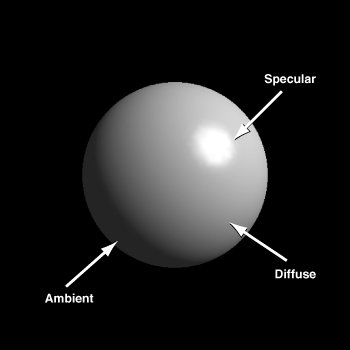
\includegraphics[width=200pt]{img/light}
    \caption{Lighting in OpenGL}
    \label{fig:lighting}
  \end{center}
\end{figure}

\textit{Ambient light} simulates indirect lighting. It illuminates all 
geometry in a scene at the same intensity.
\\
\textit{Diffuse light} illuminates a surface based on its orientation 
to a light source. OpenGL diffuse lighting adheres to 
Lambert's law, in which the amount of illumination is proportional 
to the cosine of the angle between the surface normal and the 
light vector, and the diffused light reflects equally in 
all directions.
\\
\textit{Specular light} approximates the reflection of the light source on 
a shiny surface.
\\
At first glance, controlling OpenGL lighting might appear complex. 
The amount of code required to obtain simple lighting effects, 
however, is actually quite small. That is:
\\
\begin{lstlisting}[caption={Lighting example}, label={code:lighting}]
// Enable OpenGL lighting
glEnable( GL_LIGHTING );

// Enable a single light source
glEnable( GL_LIGHT0 );
\end{lstlisting}

\texttt{GL\_LIGHT0} is one of the light points available to 
OpenGL programmers. For every light point, one can set its 
position and parameters for each light component. For example:
\\
\begin{lstlisting}[caption={Complex lighting example}, label={code:complexlighting}]
GLfloat lightpos[] = { 0.0f, 0.0f, 1.0f, 0.0f };
GLfloat lightcolor[] = { 1.0f, 1.0f, 1.0f };
GLfloat ambcolor[] = { 1.0f, 1.0f, 1.0f };

glEnable(GL_LIGHTING);
glEnable(GL_LIGHT0);                        
glLightfv(GL_LIGHT0, GL_POSITION, lightpos);
glLightfv(GL_LIGHT0, GL_AMBIENT, lightcolor);
glLightfv(GL_LIGHT0, GL_DIFFUSE, lightcolor);
glLightfv(GL_LIGHT0, GL_SPECULAR, lightcolor);
\end{lstlisting}

\clearpage
\section{Perspective in OpenGL}
\label{opengl:perspective}

Perspective in OpenGL can be something very trick to work with. 
It all starts from the definition of \textit{frustum}, as the portion
of space seen from the point of view (see \cite{wiki:frustum} 
for further information). To define the frustum we use the function
named \texttt{gluPerspective()} \cite{opengl:gluPerspective}, which takes 
four parameters.
\\
The first parameter indicates the \textit{FOV} - i.e. Field Of View -
along the Y axis, in degrees: the chosen value is 60. The
second one expresses ratio between actual width and height, 
in our case 624/442. The last two parameters specify the distance 
from the viewer to the near clipping plane and to the far one, 
according to the frustum definition.
\\
By using two close values for the far and near clipping planes 
distance the application will not be able to display 3D
objects, unless the point of view is relatively close to them. 
If we want to be able to see 3D objects as they are moving away
from the point of view, we need to increase the difference between 
the last two parameters of the \texttt{gluPerspective()} function. In
our case, the chosen values are 0.001 and 100000 (its ratio is 
equal to 10exp8).
\\
The \texttt{gluPerspective()} function affects the \textbf{projection} 
matrix, previously selected by changing matrix mode. Finally,
in order to set our point of view, we must change matrix again, 
this time to work with the \textbf{modelview} matrix.
\\
The function named
\texttt{gluLookAt()} allows to set the point of view, with its coordinates, 
the coordinates of the point to look at and its orientation.
\\
See \cite{opengl:gluLookAt} for further details.
\\
\begin{lstlisting}[caption={OpenGL perspective example}, label={code:perspective}]
  /* define the projection transformation */
  glMatrixMode(GL_PROJECTION);
  glLoadIdentity();
  gluPerspective(60, 624/442, 0.001, 100000);
  
  /* define the viewing transformation */
  glMatrixMode(GL_MODELVIEW);
  glLoadIdentity();
  gluLookAt(0.0, 0.0, 10.0,
            0.0, 0.0, 0.0,
            0.0, 1.0, 0.0);
\end{lstlisting}

